\section{Введение}

\clearpage

\section{Вибрационное погружение и внедрение}

\begin{definition}
    Вибрационным погружением называют проникновение твёрдого тела в сопротивляющуюся среду
    под действием постоянной и знакопеременной сил.
\end{definition}

\begin{definition}
    Под вибрационным внедрением будем понимать внедрение твёрдого тела в сопротивляющуюся среду с заданной
    средней скоростью.
\end{definition}

Схема вибрационного погружателя свай представлена на рис. \ref{fig:vp}.
К погружаемому элементу 1 (будем называть его \textit{сваей}) жестко присоединен \textit{вибровозбудитель} 2,
генерирующий силу $\Phi_0 \sin \omega t$. С вибровозбудителем посредством очень мягкх пружин связана пригрузка 3,
оказывающая на систему статическое воздействие весом $m_0g$.

\begin{figure}[h]
    \centering
    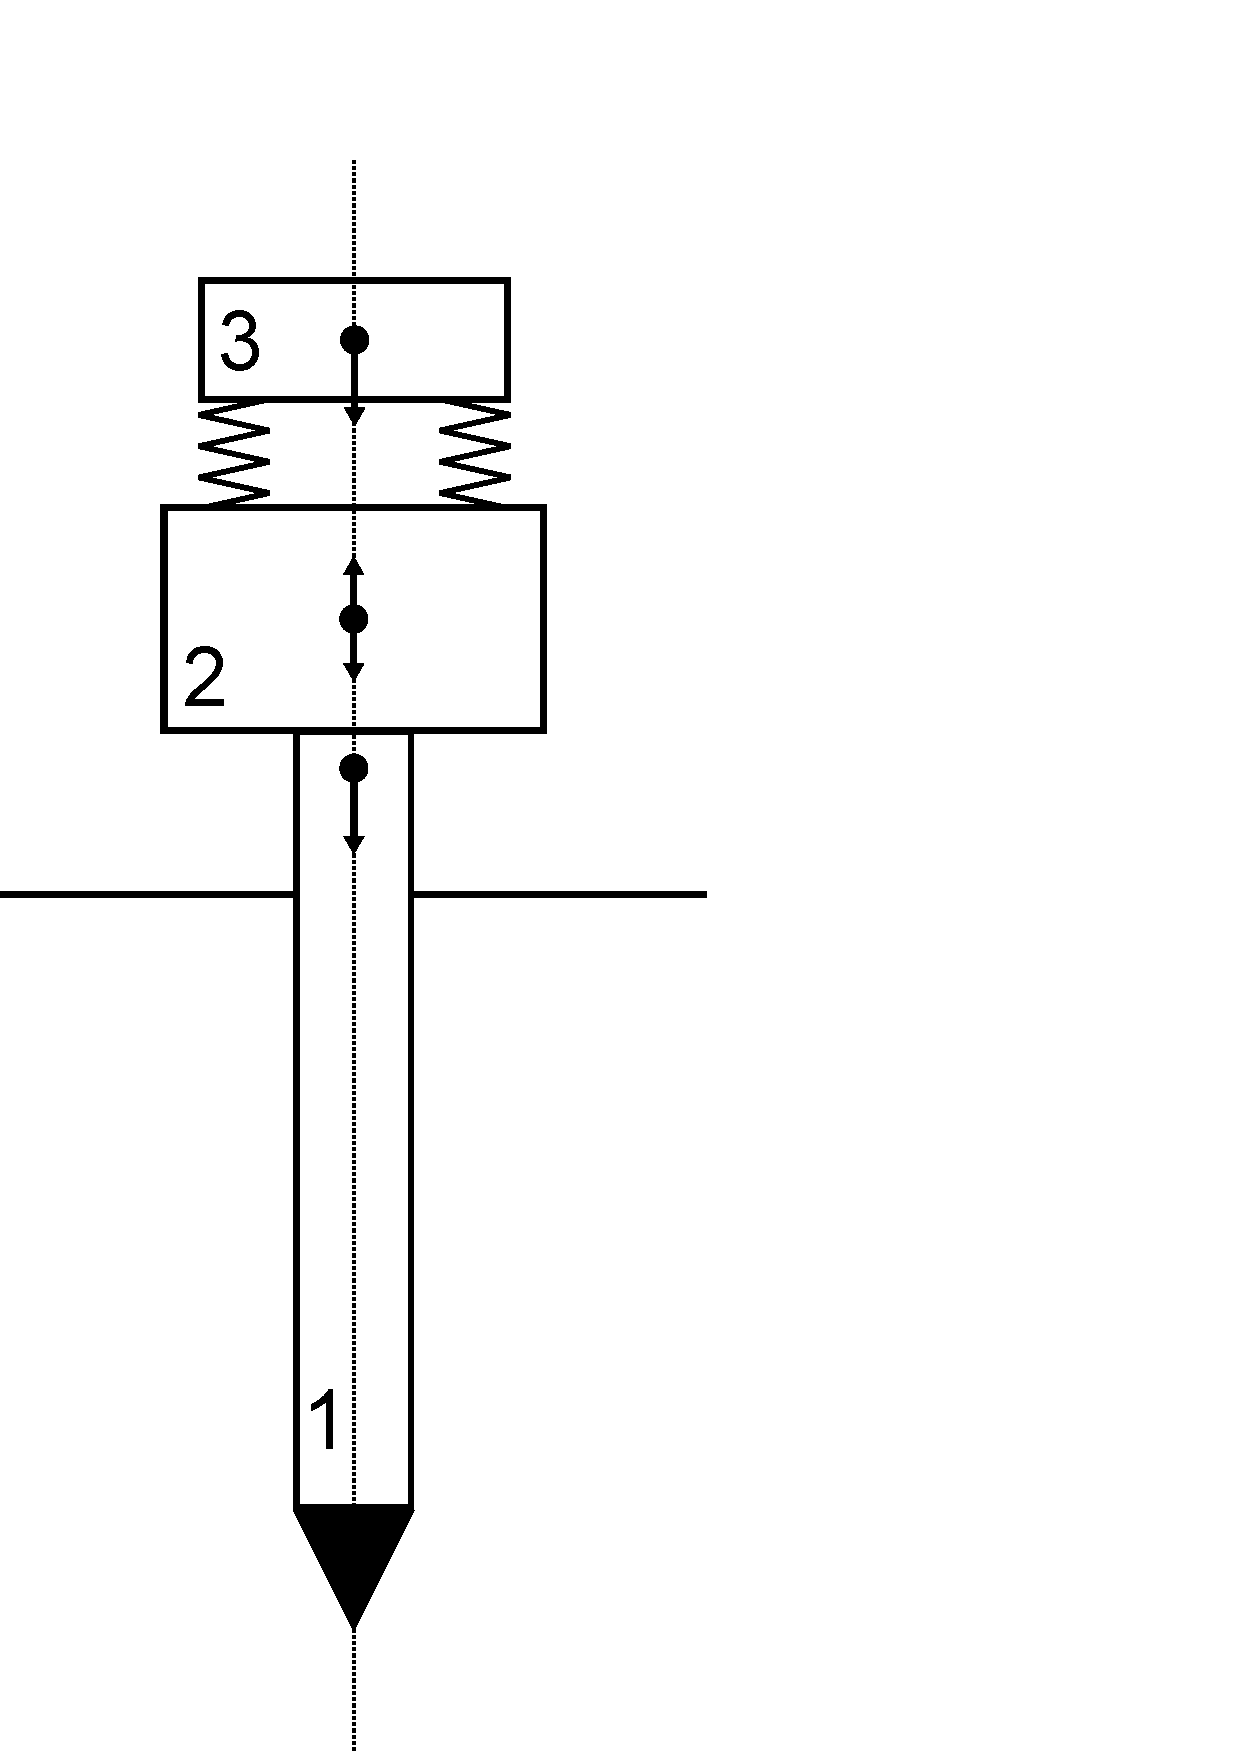
\includegraphics[width=0.3\linewidth]{pogruzhatel.png}
    \caption{Вибрационный погружатель.}
    \label{fig:vp}
\end{figure}

Дифференциальное уравнение движения сваи при сделанных предположениях имеет вид
\begin{equation}
    m_1\ddot{x} = (m_1 + m_0)g + \Phi_0 \sin \omega t + F(\dot{x}),
\end{equation}
где
\begin{equation}
    \begin{aligned}
        F(\dot{x}) =
        \begin{cases}
            -F_+ \quad \text{при} \quad \dot{x} > 0,\\
            \phantom{-}F_- \quad \text{при} \quad \dot{x} < 0,
        \end{cases}\\
        -F_+ < F(\dot{x}) < F_- \quad \text{при} \quad \dot{x} = 0.
    \end{aligned}
\end{equation}